\iffalse
\documentclass[a4paper,12pt,twocolumn]{article}
\usepackage{graphicx}
\usepackage[margin=0.5in]{geometry}
\usepackage[cmex10]{amsmath}
\usepackage{array}
\usepackage{gensymb}
\usepackage{booktabs}
\title{Conic Assignment}

\author{Ravi Sumanth Muppana- FWC22003}
\date{September 2022}
\providecommand{\norm}[1]{\left\lVert#1\right\rVert}
\providecommand{\abs}[1]{\left\vert#1\right\vert}
\let\vec\mathbf
\newcommand{\myvec}[1]{\ensuremath{\begin{pmatrix}#1\end{pmatrix}}}
\newcommand{\mydet}[1]{\ensuremath{\begin{vmatrix}#1\end{vmatrix}}}
\providecommand{\brak}[1]{\ensuremath{\left((#1\right)}}
\begin{document}
\maketitle
\section{Problem:}
<<<<<<< HEAD
Find the equation of circle with radius $5$ whose center lies on x-axis and passes through point $\brak{2,3}$.
\fi
\solution 
See Fig. 
		\ref{fig:11/11/1/12}.
	\begin{figure}[!ht]
		\centering
 \includegraphics[width=\columnwidth]{chapters/11/11/1/12/figs/conic.png}
		\caption{}
		\label{fig:11/11/1/12}
  	\end{figure}
\iffalse
=======
Find the equation of circle passing with radius $5$ whose center lies on x-axis and passes through point $(2,3)$.
>>>>>>> f531642 (Created codes and figs folder)
\maketitle
\section{Solution:}
\begin{figure}[h]
	\includegraphics[width=\linewidth]{conic.png}
\caption{Circle}
\end{figure}
\subsection{Theory:}
The circle equation when it's center and radius are given is
\begin{align}
<<<<<<< HEAD
	&\vec{(x-a)^2} + \vec{(y-b)^2} = \vec{r^2}\\
\end{align}
where the centre of the circle is $\myvec{a\\b}$.
\subsection{Mathematical Calculation:}
Given the radius of circle is $5$. The circle passes through a point $\myvec{2\\3}$. Also, the center of circle is assumed as $\myvec{a\\0}$. Substitute $\myvec{a\\0}$ in eq.$1$ we get,
\begin{align}
	&\vec{(x-a)^2} + \vec{(y)^2} = \vec{25}\\
\end{align}
As the point $\myvec{2\\3}$ passes through the circle, substitute $\myvec{2\\3}$ in the equation, we get,
\begin{align}
	&\vec{(2-a)^2} + \vec{(3)^2} = \vec{25}\\
	&\vec{4+a^2-2a} + \vec{9} = \vec{25}\\
	&\vec{a^2-2a+13} = \vec{25}\\
	&\vec{a^2-2a-12} = 0\\
\end{align}
The roots of the equation will be $(6,-2)$. Hence, the center of the circle can be $\myvec{6\\0}$ or $\myvec{-2\\0}$.
The equation of circle will therefore be,
\begin{align}
	&\vec{(x-6)^2} + \vec{y^2} = 25\\
	&\vec{(x+2)^2} + \vec{y^2} = 25
=======
	&\vec{x^Tx} + \vec{2u^Tx} + c = 0\\
	&\vec{x} = \myvec{x\\y}\\\vec{u} = \myvec{g\\f}\\
\end{align}
where the centre of the circle is $\myvec{-g\\-f}$.
\subsection{Mathematical Calculation:}
Given the radius of circle is 5, the center lies on x-axis. The circle passes through a point $\vec{P} = \myvec{2\\3}$. We can get below equations,
\fi
From the given information, the following equations can be formulated
using 
	\eqref{eq:circ-eq}.
\begin{align}
		\label{eq:11/11/1/12/1}
	\norm{\vec{P}}^2 + 2 \vec{u}^{\top}\vec{P} + f &= 0
	\\
		\label{eq:11/11/1/12/2}
	\vec{u} &= k\vec{e}_1
	\\
		\label{eq:11/11/1/12/3}
	\norm{\vec{u}}^2 - f &= r^2
\end{align}
where 
\begin{align}
	\vec{P} = \myvec{2\\3} \text{ and } r = 5
\end{align}
From 
		\eqref{eq:11/11/1/12/1}
		and 
		\eqref{eq:11/11/1/12/3},
\begin{align}
	\norm{\vec{P}}^2 + 2 \vec{u}^{\top}\vec{P} + \norm{\vec{u}}^2 &= r^2
\end{align}
Substituting from 
		\eqref{eq:11/11/1/12/2} in the above, 
\begin{align}
	k^2  + 2k \vec{e}_1^{\top}\vec{P} + \norm{\vec{P}}^2- r^2 = 0
\end{align}
resulting in 
\begin{align}
	k =  - \vec{e}_1^{\top}\vec{P} \pm \sqrt{\brak{{ \vec{e}_1^{\top}\vec{P}  }}^2 + r^2 - \norm{\vec{P}}^2 } 
\end{align}
Substituting numerical values, 
\begin{align}
	k = 2, -6
\end{align}
resulting in circles with centre
\begin{align}
	-\vec{u} = \myvec{-2 \\ 0} \text{ or } \myvec{6 \\ 0}.
\end{align}
This is verified in Fig. 
		\eqref{fig:11/11/1/12}.
\iffalse
Now,
\begin{align}
	&\myvec{0*u_x\\u_y} = \myvec{0\\0}\\
	&u_y=0\\
	&13+2\myvec{u_x\\0}\myvec{2 &3}+f = 0\\
	&\myvec{u_x\\0}\myvec{u_x &0} - f = 25
\end{align}
Solving the above yield us to the points $\myvec{-2\\0}$ and $\myvec{6\\0}$.
\begin{align}
	&\vec{x^Tx} + \vec{2u^Tx} + c = 0
\end{align}
We know that $\vec{x} = \myvec{2\\3}$ and centre $\vec{u} = \myvec{-2\\0},\myvec{6\\0}$. Substitute them.
\begin{align}
	&\vec{x^Tx} + 2\myvec{-6 &0}\vec{x} + c1 = 0\\
	&\vec{x^Tx} + 2\myvec{2 &0}\vec{x} + c2 = 0
\end{align}
The value of c is $c = g^2+f^2-r^2$. Hence c can be $11,-21$. On substitution we get, the circle equations as,
\begin{align}
	&\vec{x^Tx} + \myvec{-6 &0}\vec{x} + 11 = 0\\
	&\vec{x^Tx} + \myvec{2 &0}\vec{x} + -21 = 0\\
>>>>>>> f531642 (Created codes and figs folder)
\end{align}
\section{Construction:}

\begin{table}[h]
        \centering
\setlength\extrarowheight{2pt}
        \begin{tabular}{|c|c|c|}
                \hline
                \textbf{variable} & \textbf{length/point} & \textbf{Description}\\
                \hline
		A & np.roots(coeff) & coeff = (1,-4,-12)\\
		\hline
		c & $(a-A[0])^2+b^2-r^2$ & Circle Eqn\\
		\hline
        \end{tabular}
\end{table}
\end{document}
\fi
